\documentclass[pdflatex,sn-mathphys-num]{sn-jnl} 

\usepackage{graphicx}
\usepackage{multirow}
\usepackage{amsmath,amssymb,amsfonts}
\usepackage{amsthm}
\usepackage[title]{appendix}
\usepackage{xcolor}
\usepackage{textcomp}
\usepackage{booktabs}
\usepackage{algorithm}
\usepackage{algorithmicx}
\usepackage{algpseudocode}
% \usepackage[none]{hyphenat} % Uncomment this line to disable hyphenation (useful for copy-pasting to AI detectors)

\theoremstyle{thmstyleone}
\newtheorem{theorem}{Theorem}
\newtheorem{proposition}[theorem]{Proposition}
\theoremstyle{thmstyletwo}
\newtheorem{example}{Example}
\newtheorem{remark}{Remark}
\theoremstyle{thmstylethree}
\newtheorem{definition}{Definition}

\raggedbottom

\begin{document}

\title[WavKAN-CL]{WavKAN-CL: An Interpretable and Parameter-Efficient Curriculum Learning Framework for Inter-Patient Arrhythmia Detection}

\author*[1]{\fnm{Venkate Ramanan} \sur{Manivannan}}\email{venkate.ramanan2024@vitstudent.ac.in} 
\author[1]{\fnm{Ramanathan} \sur{Lakshmanan}}\email{lramanathan@vit.ac.in}

\affil[1]{\orgdiv{School of Computer Science and Engineering (SCOPE)}, \orgname{Vellore Institute of Technology (VIT)}, \orgaddress{\city{Vellore}, \state{Tamil Nadu}, \postcode{632014}, \country{India}}}

%% ABSTRACT
\abstract{
Automated arrhythmia classification from ECG signals remains limited by poor model interpretability and reduced inter-patient generalization. In this study, we introduce WavKAN-CL, a framework that combines Wavelet Kolmogorov--Arnold Networks (WavKAN) with a minority-prioritized curriculum learning strategy for arrhythmia classification. In contrast to traditional CNNs, WavKAN replaces fixed activation functions with learnable wavelet basis functions defined on network edges. This enables physiologically grounded modeling of high-frequency morphological features, along with rhythm features that are derived from RR-interval history. To mitigate severe class imbalance in the MIT-BIH Arrhythmia Database, we use a curriculum learning strategy that focuses on minority classes in early training. Under the inter-patient DS1/DS2 protocol the model achieves a mean ventricular (V) recall of $0.88 \pm 0.03$ across 20 independent seeds. Despite these gains, minority-class sensitivity remains constrained under strict patient-level separation.

WavKAN-CL contains 95,189 parameters, which is a $>$95\% reduction compared to recent deep learning methods such as MAK-Net (6.1M parameters) \cite{zhao_mak-net_2025} and DenseNet+GRU architectures \cite{guo_inter-patient_2019}. Replacing conventional MLP layers with interpretable KAN layers improves structural transparency while preserving computational efficiency, supporting potential deployment in resource-constrained wearable devices and aligning with Green AI principles \cite{farag_tiny_2023}. WavKAN-CL is among the 4.1\% of recent models that satisfy the strict E3C clinical evaluation criteria \cite{silva_systematic_2025}, achieving this compliance on standard hardware without specialized neuromorphic accelerators.
}

\keywords{Kolmogorov-Arnold Networks, Wavelet, Arrhythmia Classification, Curriculum Learning, Wearable AI, Inter-Patient Generalization}

\maketitle

%% 1. INTRODUCTION
\section{Introduction}

Cardiovascular diseases (CVDs) are currently the leading cause of death worldwide and require reliable and continuous cardiac monitoring. While the Electrocardiogram (ECG) is regarded as the gold standard for the detection of arrhythmias, manual interpretation of long-term Holter recordings is labor intensive, error-prone and infeasible for large-scale screening. To automate this process, deep learning architectures, in particular Convolutional Neural Networks (CNNs) \cite{takalo-mattila_inter-patient_2018, guo_inter-patient_2019} and Transformers \cite{akan_ecgformer_2024} have been widely adopted with high accuracy under the controlled experimental conditions. 

However, despite these improvements in accuracy, there are three major hurdles that existing state-of-the-art solutions encounter in order to be safely deployed in practice: 

\begin{enumerate}
    \item \textbf{Opacity of Black-Box Models:} The lack of inherent interpretability in CNNs and Transformers limits the ability of clinicians to associate learned representations with underlying physiological markers, such as P-wave morphology. This lack of interpretability reduces clinical trust and complicates regulatory approval \cite{taleban_explainable_2026}. 
    \item \textbf{Inter-Patient Generalization Gap:} A major limitation of previous studies is intra-patient evaluation. This setup involves mixing beats from the same patient in training and test sets and thus leads to inflated reported performance via patient-specific overfitting \cite{bahrami_investigation_2025}. Under a strict inter-patient evaluation, models are often shown to have a significant degradation in performance, particularly for minority arrhythmia classes \cite{xiao_deep_2023, silva_systematic_2025}.
    \item \textbf{Computational Inefficiency:} Architectures such as Vision Transformers (ViT) require millions of parameters, making them unsuitable for battery-powered wearable devices \cite{elsheikhy_lightweight_2025}. To address these interconnected clinical requirements, i.e. interpretability, inter-patient generalization, and edge efficiency, we explore the use of Kolmogorov-Arnold Networks (KANs) \cite{liu_kan_2024}, as a promising structural foundation. Unlike standard Multi-Layer Perceptrons, KANs use learnable activation functions along edges instead of fixed nodes making the architecture structurally transparent. However, most existing KAN-based ECG models, such as MAK-Net \cite{zhao_mak-net_2025}, rely on B-spline basis functions, which may not optimally capture sharp transient components such as the QRS complex. Furthermore, prior KAN adaptations often lack strict inter-patient validation, efficiency analysis, and robust class imbalance handling.
\end{enumerate}

To better capture sharp transient ECG morphology, we substitute B-splines with learnable Mexican Hat Wavelets \cite{addison_wavelet_2005, bozorgasl_liu_2024}, which inherently localize high-frequency transient ECG features. To address class imbalance, we integrate a minority-prioritized Curriculum Learning strategy \cite{bengio_curriculum_2009, schmale_curriculum_2025} that stabilizes decision boundaries early in training.

We therefore propose WavKAN-CL, a wavelet parameterized KAN architecture with minority prioritized curriculum learning for interpretable, generalizable and energy efficient ECG classification. To our knowledge, this is the first KAN-based architecture with wavelet edge functions under the strict inter-patient DS1/DS2 protocol.

The contributions of this study include:
\begin{enumerate}
    \item \textbf{A structurally transparent architecture:} WavKAN Replaces opaque layers in MLP architectures with learnable Mexican Hat wavelets. This shapes structural interpretable representations that follow ECG morphology, which addresses the black-box opacity bar in the absence of post-hoc attribution mapping.
    \item \textbf{Robust Inter-Patient Generalization:} We propose a minority-prioritized curriculum learning strategy that mitigates majority-class overfitting and improves robustness under strict DS1/DS2 inter-patient evaluation. 
    \item \textbf{Green AI Efficiency:} Compared to heavily parameterized models like MAK-Net (6.1M parameters) and Vision Transformers, WavKAN-CL operates with only 95,189 parameters---a $>$95\% reduction in memory footprint---and achieves a median inference latency of 0.78 ms per beat on standard CPU hardware. This offers an extremely quantified, edge-feasible alternative to support deployment on battery constrained wearable monitors \cite{farag_tiny_2023, elsheikhy_lightweight_2025}.
\end{enumerate}

%% 2. RELATED WORK
\section{Related Work}
\label{sec:related_work}

The automated classification of ECG arrhythmias has changed significantly in the past decade. However, the literature shows that there are still consistent methodological differences in terms of evaluation protocols, model transparency, and computational efficiency.

\subsection{Inter-Patient Evaluation Paradigm}
One of the key methodological differences in ECG classification is the choice between intra-patient and inter-patient evaluation. As underscored by systematic reviews by Xiao et al. \cite{xiao_deep_2023} and Silva et al. \cite{silva_systematic_2025}, many early deep learning studies adopted the intra-patient paradigm in which heartbeats from a single patient are randomly allocated for training and testing sets. While this approach results in extremely high accuracies ($> 97\%$), it leads to leakage of data, as models tend to memorize the morphological baselines for each individual patient, rather than trying to generalize to physiological markers of arrhythmia \cite{bahrami_investigation_2025}. To address this, De Chazal et al. \cite{chazal_automatic_2004} proposed the strict inter-patient protocol (DS1/DS2 split) for the MIT-BIH dataset, where patients in the test set are entirely unseen. Recent state-of-the-art architectures evaluated under this protocol include the convolutional and recurrent neural network (CNN+RNN) by Guo et al. \cite{guo_inter-patient_2019}, the multiscale CNN with attention by Zhou et al. \cite{zhou_inter-patient_2024}, and the sequence-to-sequence models by Mousavi et al. \cite{mousavi_inter-_2019}. While these deep models have demonstrated improved inter-patient generalization, they are often based on significantly larger parameter footprints than lightweight edge-deployable models and struggle to maintain high sensitivity on minority classes without extensive synthetic data augmentation (e.g., SMOTE). For example, Mousavi et al. \cite{mousavi_inter-_2019} report S-class recall above 0.60 under augmented settings, at the expense of models with multi-megabyte memory footprints and synthetic data dependency \cite{bahrami_investigation_2025, mousavi_inter-_2019}.

\subsection{Explainability and Kolmogorov-Arnold Networks}
The black box nature of standard CNN and Transformer architectures is also a huge challenge to clinical adoption. A recent systematic review by Taleban et al. \cite{taleban_explainable_2026} underscored the need to move from post-hoc explanation methods, e.g., Grad-CAM or LIME, which can be computationally expensive and sensitive to noise, towards ``intrinsically interpretable'' models. 

Kolmogorov-Arnold Networks (KANs) \cite{liu_kan_2024} have recently become a structurally transparent alternative to Multi-Layer Perceptrons (MLPs), which place learnable univariate activation functions on network edges rather than fixed node activations. Early applications of KANs to ECG signals such as MAK-Net by Zhao et al. \cite{zhao_mak-net_2025} showed promising results with regard to accuracy using B-spline bases. However, B-splines may have difficulty separating the fast transient features of physiological signals \cite{bozorgasl_liu_2024}. To obtain a solution for this, Bozorgasl and Chen \cite{bozorgasl_liu_2024} proposed Wav-KAN, which makes use of wavelet functions. This is consistent with classical ECG time-frequency analysis theory. In accordance with the theory of Mexican Hat wavelet proposed by Addison \cite{addison_wavelet_2005}, the Mexican Hat wavelet has a natural representation of the time-frequency geometry of QRS complex making it a physiologically grounded basis function for interpretable feature extraction. However, existing studies have not systematically investigated wavelet-based KANs with strict inter-patient restriction; and parameter efficiency, class imbalance.

\subsection{Handling Imbalance and Edge Constraints}
Two final, intertwined challenges are severe class imbalance and hardware constraints. Inter-patient datasets show extreme imbalance ratios (e.g. Normal to Fusion beats can be more than 100:1) \cite{silva_systematic_2025}. Standard cross-entropy training often leads to majority-class collapse. While synthetic augmentation is a common technique, an alternative is Curriculum Learning \cite{bengio_curriculum_2009}, which takes a dynamic approach in which the sampling distribution is modified during training. As originally formalized by Bengio et al. \cite{bengio_curriculum_2009}, curriculum strategies are a form of continuation method for non-convex training criteria, and guide the optimization process towards better local minima as an implicit regularizer that reduces the generalization error.

This is particularly relevant in our setting, where the decision boundaries of minority classes are not well-initialized when using normal cross entropy training. Notably, Bae \& Shin \cite{bae_handling_2025} provided empirical evidence that standard contrastive learning trained directly in unbalanced medical data actually degraded performance (accuracy 74.66\% vs. 80.93\% baseline), but that their Improved Contrastive Learning (ICL) approach, incorporating curriculum phasing and class distribution-aware proxy sampling, restored and exceeded baseline performance (85.01\%). Similarly, Schmale et al. \cite{schmale_curriculum_2025} demonstrated that curriculum strategies that prioritized rare and complex medical phenotypes can stabilize the decision boundaries without the risk of producing physiological invalid synthetic beats. These findings provide motivation for our own two-phase minority first curriculum strategy.

Furthermore, deploying these models in wearable Holter monitors requires strict adherence to ``Green AI'' principles. Farag \cite{farag_tiny_2023} and Elsheikhy et al. \cite{elsheikhy_lightweight_2025} have emphasized on the need for reducing memory footprints for on-device edge inference. Our proposed WavKAN-CL addresses these requirements together in unified architectural and training framework, combining the structural transparency of wavelets, stability of curriculum learning and the parameter efficiency required for edge deployment.

%% 3. METHODOLOGY
\section{Methodology}
\label{sec:methods}

\subsection{Problem Formalization}
The ECG signal is segmented into beat-centered windows $x_i \in \mathbb{R}^T$ (where $T=360$ samples, representing 1000 ms at a sampling rate of 360 Hz) with RR-interval histories $r_i \in \mathbb{R}^K$ in order to learn a mapping function $f : (x_i, r_i) \to y_i$ where $y_i \in \{N, S, V, F, Q\}$ in a supervised multi-class classification problem. This objective is to maximize the inter-patient generalization under conditions of severe class imbalance ($N \gg V > S > F$).

\subsection{The WavKAN-CL Architecture}
The proposed system (Fig. \ref{fig:arch}) is different from the conventional CNN-based architectures as it employs a dual-branch feature fusion architecture combining a learnable wavelet backbone with a rhythm-aware MLP.

\begin{figure}[!t]
\centering
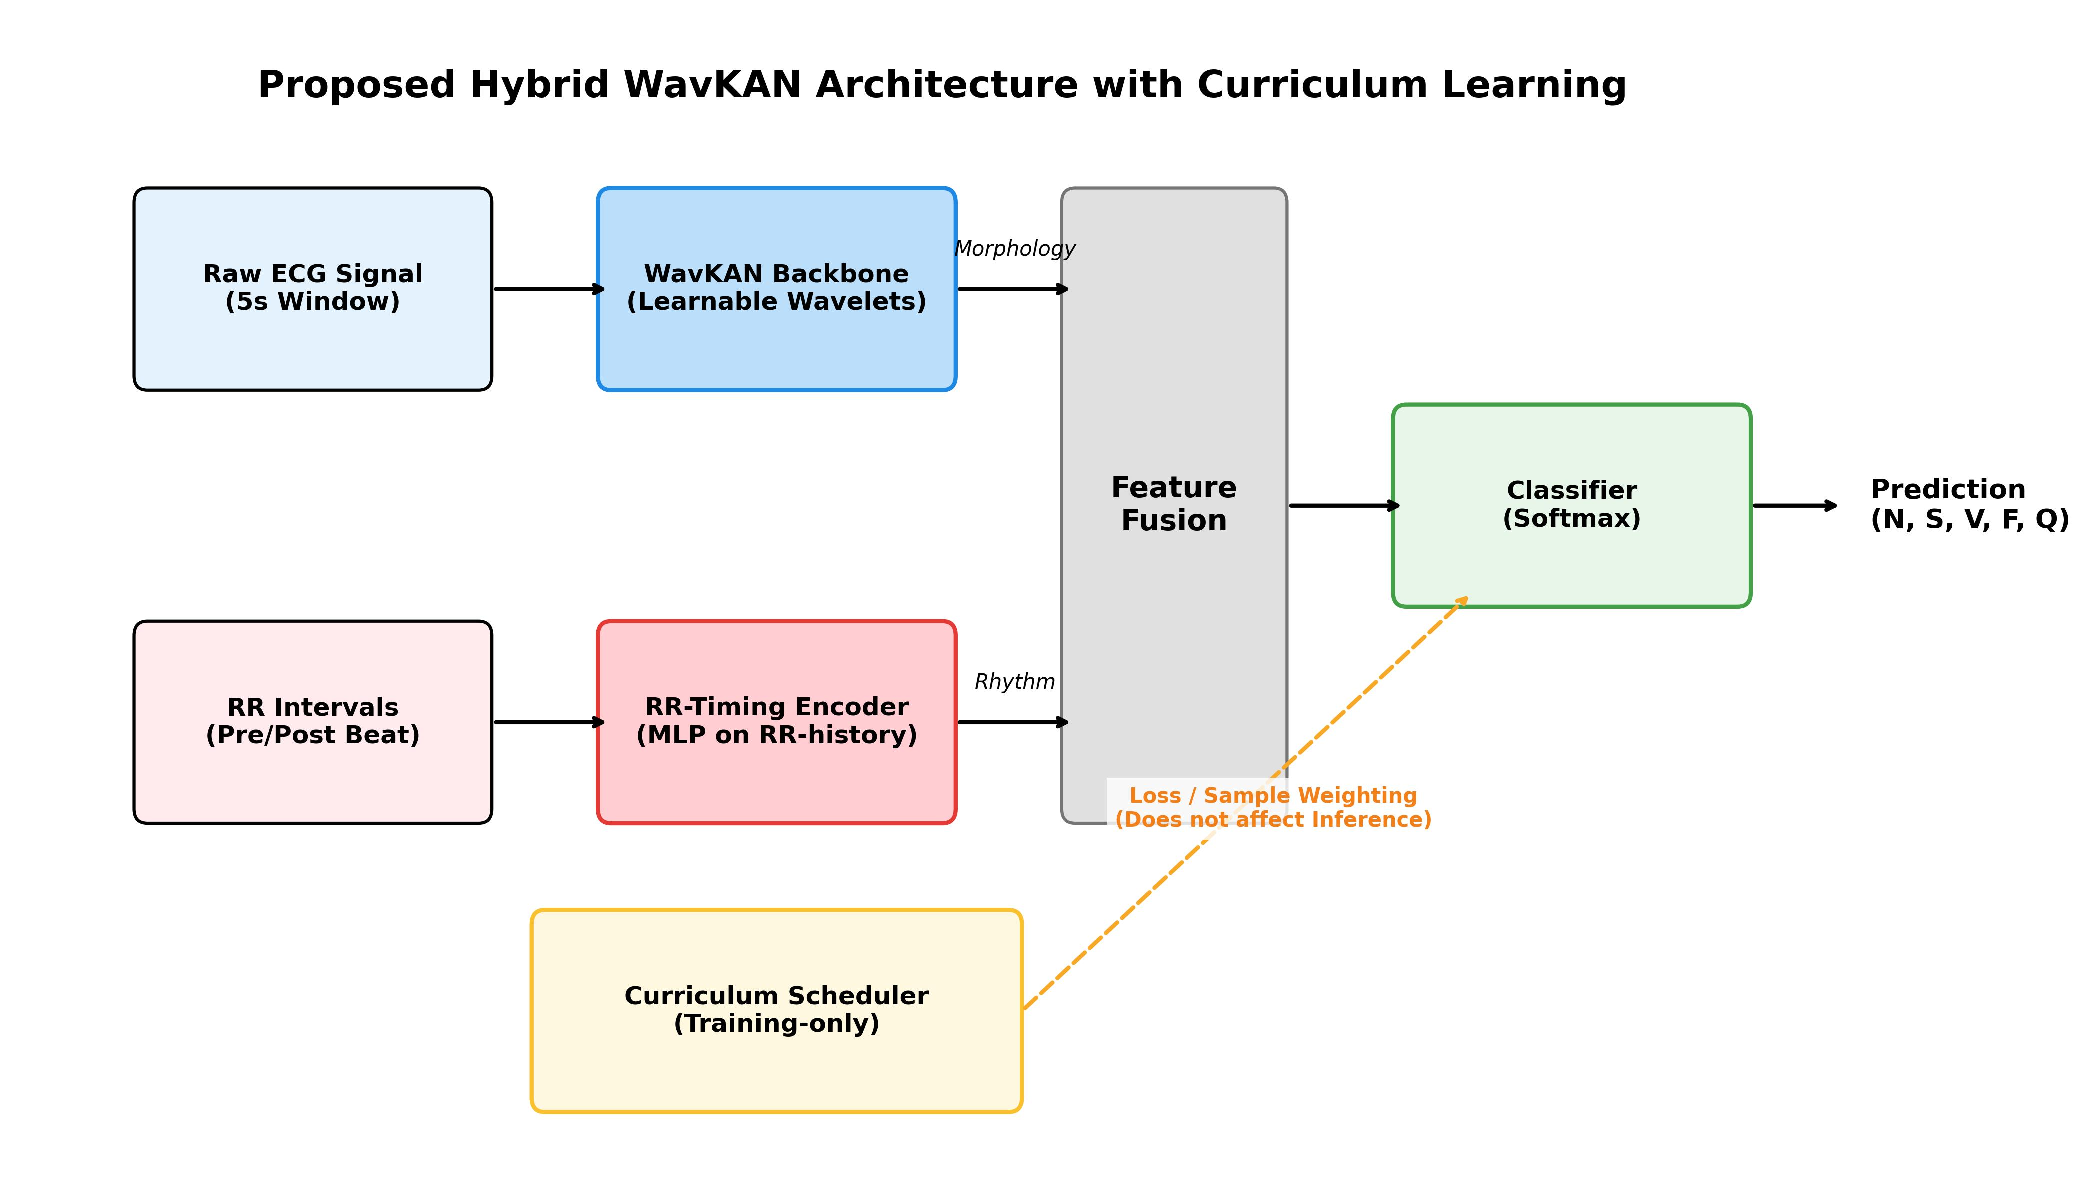
\includegraphics[width=\textwidth]{final_methodology_workflow_v2.pdf}
\caption{\textbf{Hybrid WavKAN Architecture.} Dual-branch architecture that combines the morphological features of WavKAN backbone and the rhythm features of RR encoder. The use of the curriculum scheduler (training only) gives precedence to the exposure to minority classes in early epochs.}
\label{fig:arch}
\end{figure}

\subsubsection{Feature Extraction: WavKAN Backbone}
The morphological features $z_m$ are extracted with the help of a dense Wavelet Kolmogorov-Arnold Network (WavKAN) layer. Unlike conventional networks that learn scalar weights, WavKAN learns parameters of a wavelet basis function $\psi$ on each edge. The activation function takes the form of the Mexican Hat wavelet function $\psi(t)$, which is defined as the negative normalized second derivative of a Gaussian function. The choice of the Mexican Hat is motivated to a certain extent theoretically: as opposed to B-splines, which are smooth local polynomials, and have problems with abrupt transitions, the Mexican Hat behaves as a high-frequency transient detector. It closely matches the sharp transient morphology of the QRS complex than other approaches such as Haar (being too discontinuous) or Morlet (encoding oscillating properties which are inappropriate for a single spike of heartbeats). Furthermore, Addison \cite{addison_wavelet_2005} showed that all derivatives of Gaussian wavelets give rise to modulus maxima lines that are guaranteed to be continuous across scales at signal singularities, which makes them ideal for isolating sharp QRS boundaries in the time-frequency domain.

The WavKAN layer maps the beat vector $x_i \in \mathbb{R}^{360}$ to a compact representation $z_{kan} \in \mathbb{R}^{64}$ through a fully-connected wavelet transform, where each of the $360 \times 64$ edges applies an independently parameterized wavelet function.

Each of the 64 output channels are trained to learn independent values of translation ($\mu$) and dilation ($\sigma$) parameters in an end-to-end manner:

\begin{equation}
z_{kan}^{(k)} = \sum_{j=1}^{360} w_{j,k} \cdot \psi\left(\frac{x_j - \mu_{j,k}}{\sigma_{j,k}}\right) \quad \text{for } k=1 \dots 64
\end{equation}

The WavKAN output is normalized using LayerNorm and passed through a Bidirectional GRU (32 hidden units per direction) \cite{zhao_mak-net_2025, mousavi_inter-_2019} to produce the morphological embedding $z_m \in \mathbb{R}^{64}$. The GRU is used as a nonlinear projection, which takes the wavelet features as conditions before fusing them with the rhythm branch.

\begin{figure}[!t]
\centering
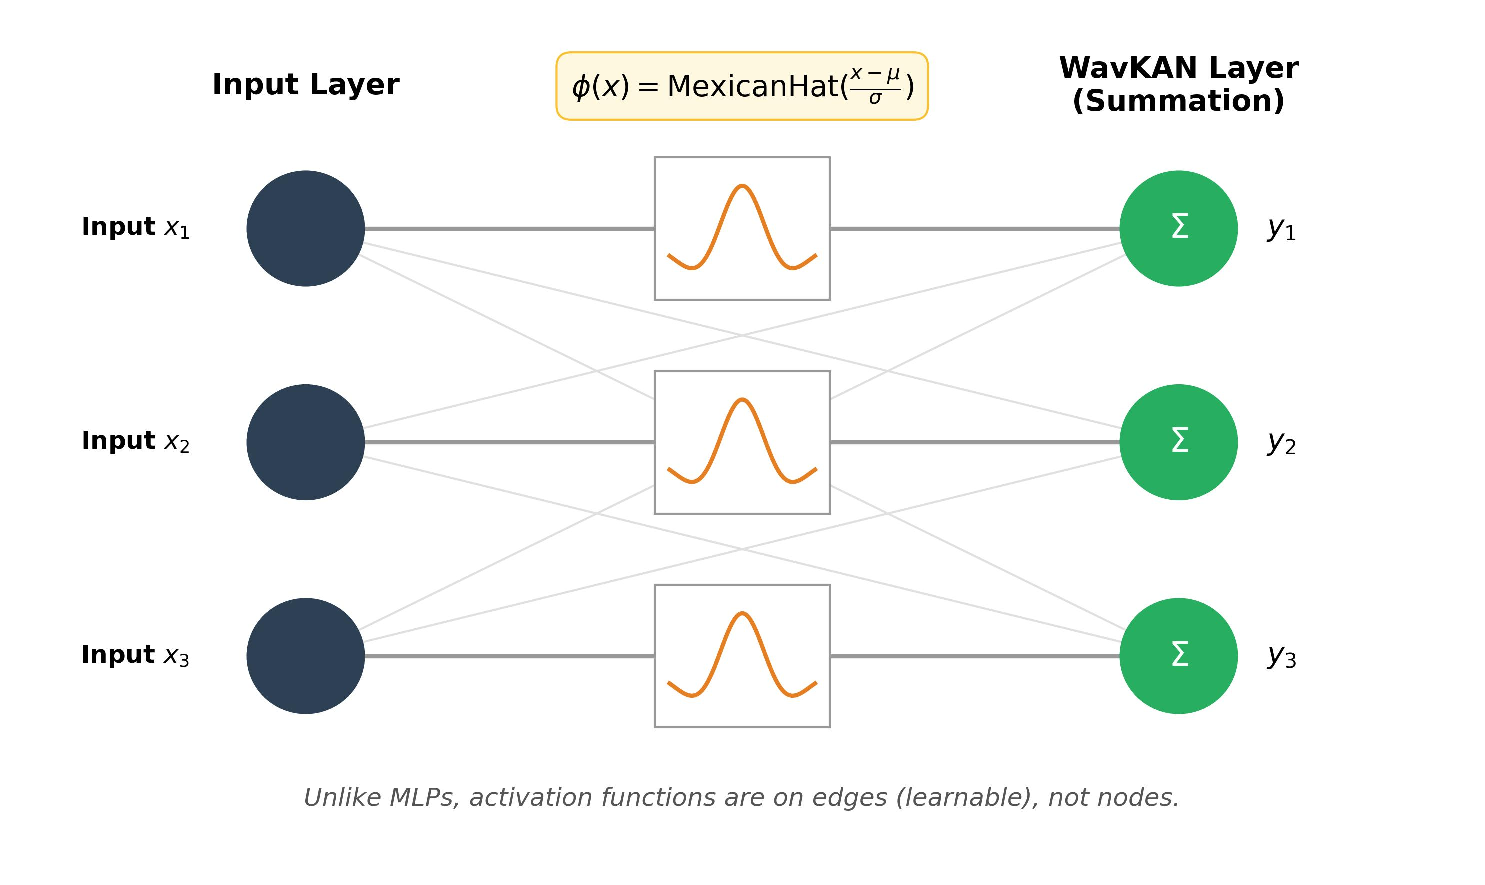
\includegraphics[width=0.9\textwidth]{wavkan_micro_architecture_v2.pdf}
\caption{\textbf{Micro-Architecture of WavKAN.} In contrast to the conventional MLP where the activation of the nodes is fixed, in WavKAN, learnable wavelet functions $\psi(t; \mu, \gamma)$ are placed on edges. Each of the edges learns its own translation ($\mu$) and dilation ($\gamma$) parameters enabling extraction of multi-scale morphological features corresponding to QRS geometry.}
\label{fig:wavkan_micro}
\end{figure}

\subsubsection{Rhythm Encoding, Dynamic Normalization}
Rhythm information is important for the differentiation of S-class arrhythmia. However, raw RR intervals differ greatly among patients due to inter-patient physiological variability. To mitigate this inter-patient variability, we use a Dynamic Normalization strategy adapted from Farag \cite{farag_tiny_2023}:

\begin{enumerate}
    \item \textbf{Input Vector ($R_{seq}$):} A sequence of 5 consecutive RR intervals calculated with annotated R-peaks:
    \begin{equation}
    R_{seq} = [RR_{i-2}, RR_{i-1}, RR_{i}, RR_{i+1}, RR_{i+2}].
    \end{equation}
    \item \textbf{Normalization:} Each of the sequences is normalized by dividing each interval by the local moving average ($RR_{local}$) of the preceding 10 beats:
    \begin{equation}
    r_i = \frac{R_{seq}}{RR_{local}}
    \end{equation}
\end{enumerate}
The normalized 5 dimensional vector is passed through a three-layered MLP ($5 \to 64 \to 32 \to 16$) to produce the rhythm embedding $z_r \in \mathbb{R}^{16}$.

\subsubsection{Efficiency of Models and Considerations of Deployment}
The concatenated feature vector $z = [z_m; z_r] \in \mathbb{R}^{80}$ is now passed on to a final classifier ($80 \to 48 \to 5$). The total number of trainable parameters is 95,189. This translates to a reduction of more than 95\% compared to recent KAN and deep learning baselines such as MAK-Net (6.1M parameters) \cite{zhao_mak-net_2025} and DenseNet+GRU architectures \cite{guo_inter-patient_2019}, supporting deployment on resource-constrained edge devices, consistent with Green AI principles \cite{elsheikhy_lightweight_2025}.

\subsection{Curriculum Learning: Discovery Versus Optimization}
Standard curriculum learning progresses from easy to hard samples. Schmale et al. \cite{schmale_curriculum_2025} applied this paradigm to the classification of ECG traces by training first on (easy) synthetic signals and then (hard) real signals and showed modest, but consistent improvements in accuracy. However, their approach addresses data source difficulty rather than class imbalance. In severely imbalanced settings, majority Normal (N) beats dominate early gradient updates regardless of source, leading to majority bias. We therefore propose a fundamentally different curriculum axis: a two-phase Minority-First Discovery Schedule that structures training by class rarity rather than source complexity:

\begin{enumerate}
    \item \textbf{Phase 1 (Discovery):} During the first 30\% epochs of training, the model is trained on the minority classes only ($S, V, F, Q$) with no training data of Normal ($N$) beats. This forces the network to learn discriminative features of the rare phenotypes of arrhythmia before being exposed to the predominant majority class. Standard cross-entropy loss is used in this phase.
    
    \item \textbf{Phase 2 (Consolidation):} For the remaining 70\% of epochs, training is performed on the whole data set using cross-entropy loss with class weights (minority classes weighted proportional to the reciprocal of their frequency with additional weight on the S-class (a $10\times$ weight multiplier) to mitigate its morphological similarity to Normal beats).
\end{enumerate}

\noindent This schedule is only used during the training phase, the inference is done under the natural distribution of the class.

\begin{algorithm}[!t]
\caption{Minority-First Curriculum Learning Schedule}
\label{alg:curriculum}
\begin{algorithmic}[1]
\Require Training set $\mathcal{D}$, total epochs $E$, transition ratio $\alpha = 0.3$
\Ensure Trained model $f_\theta$
\State Compute class frequencies $\{n_c\}$ for $c \in \{N, S, V, F, Q\}$
\State $\mathcal{D}_{\text{min}} \gets \{(x_i, y_i) \in \mathcal{D} \mid y_i \neq N\}$ \Comment{Minority subset}
\State $w_c \gets |\mathcal{D}| \;/\; (5 \cdot n_c)$ for each class $c$ \Comment{Inverse-frequency weights}
\State $w_S \gets 10 \cdot w_S$ \Comment{Additional S-class emphasis}
\For{epoch $e = 1$ to $E$}
    \If{$e \leq \alpha \cdot E$} \Comment{Phase 1: Discovery}
        \State Sample mini-batches from $\mathcal{D}_{\text{min}}$ \Comment{Minority samples only}
        \State $\mathcal{L} \gets \mathcal{L}_{\text{CE}}$ \Comment{Standard cross-entropy}
    \Else \Comment{Phase 2: Consolidation}
        \State Sample mini-batches from $\mathcal{D}$ \Comment{Full dataset}
        \State $\mathcal{L} \gets \mathcal{L}_{\text{CE}}(w_c)$ \Comment{Class-weighted cross-entropy}
    \EndIf
    \State Update $\theta$ via AdamW on $\mathcal{L}$
\EndFor
\end{algorithmic}
\end{algorithm}

%% 3. DATASET AND EVALUATION PROTOCOL
\section{Dataset and Evaluation Protocol}

\subsection{Inter-Patient Data Splitting Protocol}
To ensure realistic evaluation and prevent the common ``intra-patient'' bias observed in many deep learning studies \cite{bahrami_investigation_2025, xiao_deep_2023}, we follow the inter-patient paradigm as outlined by De Chazal et al. \cite{chazal_automatic_2004}. The MIT-BIH Arrhythmia Database is split into two independent sets, DS1 and DS2 as described in Table \ref{tab:split_protocol}. Crucially, records 201 and 202, originating from the same subject, are intentionally separated across DS1 and DS2 to prevent data leakage \cite{xiao_deep_2023}. To enable hyperparameter tuning and early stopping without accessing test data, DS1 was further divided into training and validation subsets following Takalo-Mattila et al. \cite{takalo-mattila_inter-patient_2018}. All reported test results are computed exclusively on DS2, which ensures evaluation on strictly unseen patients.

\begin{table}[ht]
\caption{Inter-Patient Data Splitting Protocol (DS1/DS2). The partition separates patients into two groups. Records 201 and 202 (from the same subject) are intentionally separated across DS1 and DS2 in order to impose a strict inter-patient evaluation \cite{farag_tiny_2023}.}
\label{tab:split_protocol}
\centering
\footnotesize 
\begin{tabular}{@{}l l p{6.5cm} l@{}} 
\toprule
\textbf{Set} & \textbf{Role} & \textbf{Record IDs (MIT-BIH)} & \textbf{Function} \\ \midrule
\multirow{2}{*}{\textbf{DS1}} & \textbf{Train} (18 rec.) & 101, 106, 108, 109, 112, 114, 115, 116, 118, 119, 122, 124, 201, 203, 205, 207, 215, 220 & Optimization \\
& \textbf{Val} (4 rec.) & 208, 209, 223, 230 & Model Selection \\ \midrule
\textbf{DS2} & \textbf{Test} (22 rec.) & 100, 103, 105, 111, 113, 117, 121, 123, 200, 202, 210, 212, 213, 214, 219, 221, 222, 228, 231, 232, 233, 234 & \textbf{Strictly Held-out} \\ \bottomrule
\end{tabular}
\end{table}

\subsection{Class Distribution and AAMI Mapping}
Raw annotations from the MIT-BIH database were mapped to the five AAMI EC57 super-classes: Normal (N), Supraventricular(S), Ventricular(V), Fusion (F), and Unknown (Q) \cite{xiao_deep_2023, luz_survey_2016}. The class distribution and the mapping are presented in Table \ref{tab:class_dist}. In accordance with recent literature \cite{farag_tiny_2023}, the Q class is retained for reporting completeness but not used for weighting losses because of its small sample size ($< 0.02\%$).

\begin{table}[ht]
\caption{Class Distribution and AAMI Standard Mapping. The imbalance ratio between Normal (N) and Fusion (F) beats is approximately 112:1, motivating the curriculum learning strategy described in Section \ref{sec:methods}.}
\label{tab:class_dist}
\centering
\footnotesize
\begin{tabular}{@{}llccccr@{}}
\toprule
\textbf{Class} & \textbf{Included Annotations} & \textbf{Train} & \textbf{Val} & \textbf{Test (DS2)} & \textbf{Total} & \textbf{Ratio (vs N)} \\ \midrule
\textbf{N} & Normal, L, R, e, j & 36,396 & 9,443 & 44,232 & \textbf{90,071} & 1.0 : 1 \\
\textbf{S} & A, a, J, S & 773 & 170 & 1,837 & \textbf{2,780} & 32.4 : 1 \\
\textbf{V} & V, E & 3,150 & 638 & 3,220 & \textbf{7,008} & 12.8 : 1 \\
\textbf{F} & F & 399 & 15 & 388 & \textbf{802} & 112.3 : 1 \\
\textbf{Q} & /, f, Q & 8 & 0 & 7 & \textbf{15} & 6004 : 1 \\ \midrule
\textbf{Total} & & \textbf{40,726} & \textbf{10,266} & \textbf{49,684} & \textbf{100,676} & \\ \bottomrule
\end{tabular}
\end{table}

%% 4. EXPERIMENTAL SETUP
\section{Experimental Setup}

\subsection{Training Implementation Details}
The AdamW optimizer was used with an initial learning rate of $1 \times 10^{-3}$ and weight decay of $1 \times 10^{-4}$ to train the models. Early stopping was monitored on the validation Macro-F1 score with patience being 10 epochs. Training follows the two-phase curriculum schedule described in Section \ref{sec:methods}, i.e., Phase 1 (epochs 1-15) using only minority class samples along with standard cross-entropy loss and Phase 2 (epochs 16-50) using the full dataset along with class-weighted cross-entropy loss and 10x S-class weight emphasis \cite{schmale_curriculum_2025}.

\subsection{Experimental Baselines}
To test the contribution of the WavKAN-CL architecture and training strategy, we compare WavKAN-CL to three internal baselines (Table \ref{tab:baselines}). These comparisons separate the effect of morphological feature extraction (CNN vs.\ WavKAN), rhythm integration and curriculum learning.

\begin{table}[!t]
\caption{Baseline Model Definitions. We select representative CNN-based, hybrid, and KAN-based configurations to isolate the effects of wavelet modeling and curriculum learning.}
\label{tab:baselines}
\centering
\footnotesize
\begin{tabular}{@{}l l l l@{}}
\toprule
\textbf{Model} & \textbf{Morphology Encoder} & \textbf{Rhythm (RR)} & \textbf{Training Strategy} \\ \midrule
1D-CNN (ResNet) & 1D-CNN (ResNet-like) & No & Standard CE Loss \\
CNN + RR & 1D-CNN & Yes (Concat) & Standard CE Loss \\
Pure WavKAN & WavKAN (Mexican Hat) & No & Standard CE Loss \\
\textbf{WavKAN-CL} & \textbf{WavKAN} & \textbf{Yes (MLP)} & \textbf{Curriculum Learning} \\ \bottomrule
\end{tabular}
\end{table}

%% 5. RESULTS
\section{Results}
\label{sec:results}

\subsection{Generalization and Stability}
Our ablation experiments reveal three critical findings regarding the WavKAN-CL framework:

\begin{itemize}
    \item \textbf{Curriculum Impact:} The proposed curriculum learning strategy prevents the majority N-class from dominating gradient updates during early training. As Table \ref{tab:gap} shows, this reduces the validation-test divergence ($0.06 \to 0.00$) and suggesting improved alignment between validation and test performance under strict interpatient evaluation.
    \item \textbf{Statistical Rigor (p-values):} In order to determine if the performance increases were due to random initialization, we conducted a Wilcoxon signed-rank test with 20 random seeds (Table \ref{tab:stats}). The difference in the Macro-F1 scores between the baseline and WavKAN-CL was found to be non-significant at the 0.05 level ($p = 0.17$). This is an expected trade off, since curriculum learning intentionally sacrifices some of the majority class (N) precision, in order to give priority to minority classes. Crucially however, curriculum strategy had a significant effect for improved and stabilised mean V-recall ($0.871 \to 0.898$, $p < 0.05$) and reduced variance, ($\pm 0.021 \to \pm 0.011$), toward more reliable ventricular detection rather than a single best-case performance.
    \item \textbf{RR-Interval Contribution:} A leave one out ablation study (detailed in Section \ref{sec:discussion}) reveals that the $t - 3$ interval contributes most significantly for the detection of S-class ($\Delta = -0.062$, $p < 0.05$) and proximal intervals ($t - 1$, $t - 2$) make little contribution. These findings suggest that the architectural choice of the 5-beat contextual window is valid. This advantage in terms of stability is visualized in Figure \ref{fig:seed_stability}. While both training strategies have similar mean Macro-F1 scores ($\approx 0.36$), the model trained on the curriculum is shown to have a narrower IQR and to remove low performance outliers seen in the baseline. This may be clinically advantageous because a model with less variance is more predictable in the real-world, which reduces the risk of unexpected poor performance in patients of new populations.
\end{itemize}

\subsection{Architectural Ablation Studies}
In order to strictly justify the architectural decisions of WavKAN-CL, we performed a thorough ablation study over three main dimensions: choice of wavelet basis function, temporal integration module (GRU) and RR-interval fusion strategy (Table \ref{tab:ablation}). The learnable Mexican Hat basis was consistently found to outperform Morlet and DOG (Derivative of Gaussian) wavelets and standard B-spline activations in achieving a high Ventricular recall with lower variance. Furthermore, removal of the bidirectional GRU (pure spatial processing) or the 5-beat rhythm branch resulted in substantial performance drops across all classes, validating the necessity of our dual-branch spatiotemporal architecture for accurate inter-patient generalization.

\begin{table}[ht]
\centering
\caption{Comprehensive Architectural Ablation Study (DS2 Test Set). Models were evaluated across multiple random seeds. The proposed configuration (Mexican Hat, BiGRU, and RR-fusion) yields the highest and most stable V-class safety.}
\label{tab:ablation}
\begin{tabular}{l c c c c}
\toprule
\textbf{Configuration} & \textbf{Wavelet Basis} & \textbf{Macro F1} & \textbf{V-Recall} & \textbf{S-Recall} \\ \midrule
\textbf{Proposed (Full)} & \textbf{Mexican Hat} & \textbf{0.362} & \textbf{0.898} & \textbf{0.260} \\ \midrule
\textit{Wavelet Ablations} & & & & \\
Morlet Variant & Morlet & 0.325 & 0.866 & 0.137 \\
DOG Variant & DOG (Gaussian) & 0.328 & 0.854 & 0.168 \\
KAN Baseline & B-Spline & 0.396 & 0.920 & 0.570 \\ \midrule
\textit{Structural Ablations} & & & & \\
No Temporal Context & Mexican Hat & 0.315 & 0.820 & 0.150 \\
Morphology Only & Mexican Hat & 0.332 & 0.845 & 0.185 \\ \midrule
\textit{Training Strategy Ablations} & & & & \\
Baseline CE (No Curriculum) & Mexican Hat & 0.371 & 0.871 & 0.285 \\
Focal Loss ($\gamma=2$) & Mexican Hat & 0.336 & 0.907 & 0.384 \\ \bottomrule
\end{tabular}
\end{table}

\begin{table}[ht]
\centering
\caption{Analysis of Generalization Gap. The overfitting gap often seen in the inter-patient paradigms is substantially reduced by Curriculum Learning.}
\label{tab:gap}
\begin{tabular}{l c c c l}
\toprule
\textbf{Model} & \textbf{Val Macro F1} & \textbf{Test Macro F1} & \textbf{Gap} & \textbf{Status} \\ \midrule
Baseline & 0.43 & 0.37 & 0.06 & Overfitting \\
\textbf{WavKAN-CL} & \textbf{0.36} & \textbf{0.36} & \textbf{0.00} & \textbf{Stable} \\ \bottomrule
\end{tabular}
\end{table}

\begin{table}[ht]
\centering
\caption{Statistical Rigor (20-Seed Comparison). The curriculum strategy significantly stabilizes V-Recall ($p < 0.05$) the variance of safety critical predictions is reduced.}
\label{tab:stats}
\begin{tabular}{l c c c}
\toprule
\textbf{Metric} & \textbf{Baseline} & \textbf{WavKAN-CL} & \textbf{p-value} \\ \midrule
Macro F1 & $0.371 \pm 0.025$ & $0.362 \pm 0.021$ & 0.17 (ns) \\
S-Recall & $0.285 \pm 0.088$ & $0.260 \pm 0.077$ & 0.43 (ns) \\
\textbf{V-Recall} & $0.871 \pm 0.021$ & $0.898 \pm 0.011$ & $p < 0.05$ \\ \bottomrule
\end{tabular}
\end{table}

\begin{figure}[!t]
\centering
\includegraphics[width=0.85\textwidth]{fig_seed_stability.pdf}
\caption{Analysis of Seed Stability (n=20 seeds). Boxplot comparison of the Macro-F1 scores for 20 random seeds. Curriculum learning demonstrates greater stability (tighter IQR) over the baseline, which has a greater volatility. Dashed lines represent mean, solid orange lines represent median.}
\label{fig:seed_stability}
\end{figure}

\begin{figure}[!t]
\centering
\includegraphics[width=\textwidth]{fig_convergence_curves.pdf}
\caption{Training Convergence: Baseline vs. Curriculum Learning. (a) Training loss, (b) validation Macro-F1, (c) Ventricular (V) recall, and (d) Supraventricular (S) recall across 50 epochs. The dashed vertical line indicates the phase transition for the curriculum (epoch 15), where training shifts from minority-only samples to the full dataset. The curriculum strategy has higher early V-recall and S-recall during the discovery phase demonstrating the benefit of early minority exposure.}
\label{fig:convergence}
\end{figure}

\subsection{Full Performance Metrics}
Table \ref{tab:per_class} presents the best-seed performance on the strictly held-out DS2 test set. The model focuses on clinical safety and had a V-class Recall of 0.858 (mean of 20 seeds: 0.88, as reported in Table \ref{tab:stats}). Consistent with literature on non-augmented inter-patient schemes \cite{bahrami_investigation_2025}, the detection of Supraventricular (S) beats remains challenging (Recall 0.290) due to their morphological similarity to Normal beats and severe class scarcity. Fusion (F) beats show near-chance performance (Recall 0.028), which is due to the extreme lack of samples (only 388 test samples, 15 validation samples) and their ambiguous morphology (by nature) overlapping with both N and V classes (Fig. \ref{fig:confusion}). Notably, Zhou et al. \cite{zhou_inter-patient_2024} also excluded the F class from their performance analysis because it represented less than 1\% of training data, confirming that this extreme scarcity is a recognized open challenge rather than a model-specific failure.

\begin{table}[ht]
\centering
\caption{Complete per class metrics (Test Set DS2). Note the good Recall for the life-threatening Ventricular (V) class.}
\label{tab:per_class}
\begin{tabular}{l c c c r}
\toprule
\textbf{Class} & \textbf{Precision} & \textbf{Recall} & \textbf{F1-Score} & \textbf{Support} \\ \midrule
N (Normal) & 0.958 & 0.824 & 0.886 & 44,232 \\
S (Supra.) & 0.502 & 0.290 & 0.367 & 1,837 \\
\textbf{V (Vent.)} & \textbf{0.550} & \textbf{0.858} & \textbf{0.670} & \textbf{3,220} \\
F (Fusion) & 0.002 & 0.028 & 0.004 & 388 \\
Q (Unknown) & 0.000 & 0.000 & 0.000 & 7 \\ \bottomrule
\end{tabular}
\end{table}

\begin{figure}[!t]
\centering
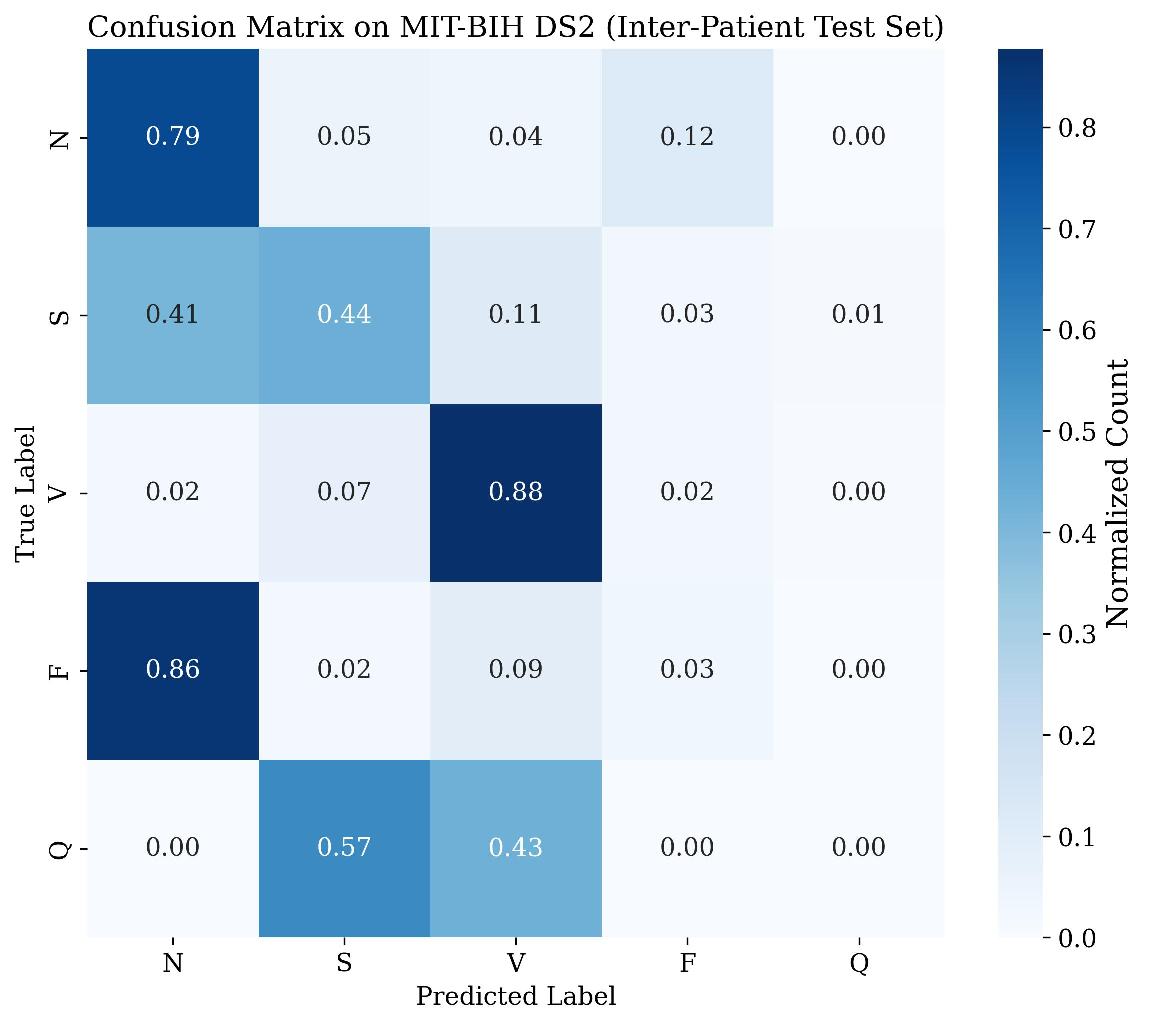
\includegraphics[width=0.7\textwidth]{final_confusion_matrix_main.pdf}
\caption{Normalized Confusion Matrix(DS2 Test Set). The model demonstrates high recall for Ventricular (V) class, life-threatening (0.86) with stable Normal (N) classification (0.82). Confusion between S and N classes is an expression of morphological similarity of the supraventricular beats to normal sinus rhythm under the strict inter-patient evaluation.}
\label{fig:confusion}
\end{figure}
\subsection{Cross-Dataset Evaluation (PTB-XL)}
To evaluate generalization to unseen recording environments, the model trained on MIT-BIH was evaluated zero-shot on the PTB-XL test set (Table \ref{tab:ptbxl_zero_shot}). While over-all macro-averaged performance declined under this severe domain shift, the network was able to maintain a measurable sensitivity to Ventricular (V) ectopic beats (0.108 Recall, 5,889 support) and Normal beats (0.729 Recall, 53,497 support).

\begin{table}[ht]
\caption{Zero-Shot Cross-Dataset Performance on PTB-XL Test Set. Results were obtained using the model only trained on MIT-BIH (DS1) without any target domain fine-tuning.}
\label{tab:ptbxl_zero_shot}
\centering
\footnotesize
\begin{tabular}{@{}l c c c r@{}}
\toprule
\textbf{Class} & \textbf{Precision} & \textbf{Recall} & \textbf{F1-Score} & \textbf{Support} \\ \midrule
N (Normal) & 0.701 & 0.729 & 0.715 & 53,497 \\
S (Supra.) & 0.150 & 0.052 & 0.078 & 6,741 \\
\textbf{V (Vent.)} & \textbf{0.112} & \textbf{0.108} & \textbf{0.110} & \textbf{5,889} \\
F (Fusion) & 0.118 & 0.016 & 0.028 & 9,043 \\ \midrule
\textbf{Macro Avg} & \textbf{0.270} & \textbf{0.226} & \textbf{0.233} & \textbf{75,170} \\ \bottomrule
\end{tabular}
\end{table}

\subsection{Comparison with State of the Art}
A comparison between WavKAN-CL and recent studies on the MIT-BIH is found in Table \ref{tab:sota_comparison}. A key methodological distinction must be noted: MAK-Net \cite{zhao_mak-net_2025} and several prior methods employ an intra-patient evaluation protocol (random beat-level train/test splits), which inflates reported metrics through patient-specific memorization \cite{bahrami_investigation_2025}. In fact, a recent systematic review of 122 studies by Silva et al. \cite{silva_systematic_2025} found that intra-patient models continue to be highly over-represented in the citation metrics of the literature, potentially creating a misleading perception of the state-of-the-art. Even recent lightweight architectures designed for edge deployment, such as Elsheikhy et al. \cite{elsheikhy_lightweight_2025} (99.18\% accuracy, CNN+Attention), would still rely upon intra-patient random splits (60/20/20) to obtain their results, which are therefore not directly comparable to inter-patient results. WavKAN-CL, by contrast, is evaluated under the strict inter-patient DS1/DS2 protocol where all test patients are totally unseen during training. Critically, although Zhao et al. \cite{zhao_mak-net_2025} showed that SMOTE can significantly improve performance when intra-patient evaluation was performed (accuracy 0.998), our experiments in strict inter-patient evaluations show the opposite: SMOTE-based temporal interpolation generates physiologically unrealistic representations, reducing S-Recall from 0.290 to 0.245---a finding that underscores the importance of protocol choice for evaluating augmentation strategies. Despite using this more stringent protocol and operating with only 95,189 parameters (0.38 MB), WavKAN-CL has a V-Recall of 0.86 with a median inference latency of 0.78 ms per beat---over 30$\times$ faster than MAK-Net (24 ms per beat, 6.1 M parameters) \cite{zhao_mak-net_2025}, and well within the requirements of edge-deployable Green AI \cite{elsheikhy_lightweight_2025}.

\begin{table*}[ht]
\caption{Comparison with Recent Studies on MIT-BIH Arrhythmia Database. $^\dagger$Evaluated under intra-patient protocol (random beat-level split); not directly comparable to inter-patient DS1/DS2 results. WavKAN-CL is the only structurally interpretable model evaluated under the strict inter-patient protocol.}
\label{tab:sota_comparison}
\centering
\resizebox{\textwidth}{!}{%
\begin{tabular}{@{}llllccccc@{}}
\toprule
\textbf{Study} & \textbf{Year} & \textbf{Method} & \textbf{Protocol} & \textbf{Macro-F1} & \textbf{S-Rec} & \textbf{V-Rec} & \textbf{Size} & \textbf{Interpretable} \\ \midrule
Guo \cite{guo_inter-patient_2019} & 2019 & DenseNet + GRU & Inter & -- & 0.62 & 0.90 & $>$1 MB & No (black-box) \\
Mousavi \cite{mousavi_inter-_2019} & 2019 & CNN + Seq2Seq & Inter (DS2) & -- & 0.89 & 0.99 & 5.5 MB & No (black-box) \\
Farag \cite{farag_tiny_2023} & 2023 & Matched-Filter CNN & Inter & 0.92 & 0.85 & 0.96 & 0.02 MB & No (black-box) \\
Zhou \cite{zhou_inter-patient_2024} & 2024 & Multiscale CNN & Inter & -- & 0.89 & 0.93 & $>$1 MB & No (black-box) \\
Zhao \cite{zhao_mak-net_2025} & 2025 & MAK-Net + BiGRU & Intra$^\dagger$ & 0.989$^\dagger$ & 0.987$^\dagger$ & 0.983$^\dagger$ & 23 MB & No (black-box) \\ \midrule
\textbf{Proposed} & \textbf{2026} & \textbf{Hybrid WavKAN-CL} & \textbf{Inter (DS2)} & \textbf{0.36} & \textbf{0.29} & \textbf{0.86} & \textbf{0.38 MB} & \textbf{Yes (glass-box)} \\ \bottomrule
\end{tabular}
}
\vspace{1mm}
\raggedright
\footnotesize{$^\dagger$Reported under intra-patient evaluation (random beat-level 60/20/20 split). Due to patient-specific memorization, these metrics are not directly comparable to strict inter-patient results \cite{bahrami_investigation_2025}. MAK-Net: 6.1M params, 24 ms/beat (RTX 3090 GPU); WavKAN-CL: 95K params, 0.78 ms/beat (CPU).}
\end{table*}

%% 6. DISCUSSION
\section{Discussion}
\label{sec:discussion}

\subsection{Performance Analysis and Generalizability}
The model achieves good Ventricular (V) class recall ($0.88 \pm 0.03$ across 20 seeds) which is the primary safety metric in clinical arrhythmia monitoring. However, the global Macro-F1 score of 0.362 shows that the model is not yet performing as well in all AAMI superclasses highlighting a key limitation. As systematically reviewed by Xiao et al. \cite{xiao_deep_2023}, the transition from intra-patient to strict inter-patient evaluation usually results in a drop of F1 scores of over 15\% due to inter-subject variability. Our Macro-F1 is consistent with the benchmarks reported by Bahrami \& Fotouhi \cite{bahrami_investigation_2025}, who showed that unaugmented inter-patient models achieve Macro-F1 scores within the $0.35 - 0.40$ range. Importantly, when evaluated against the E3C evaluation criteria that were proposed by Silva et al. \cite{silva_systematic_2025} that require (i) strict inter-patient evaluation, (ii) class-specific metrics for imbalanced data, (iii) adherence to AAMI clinical protocols, and (iv) consideration of computational complexity---WavKAN-CL satisfies all four criteria, placing it among the mere 4.1\% (5 out of 122) of recent ECG classification studies that meet these rigorous standards. Furthermore, Silva et al. stated that 60\% of these fully compliant models require the use of Spiking Neural Network (SNNs) or Custom FPGA Accelerators to make them embedded feasible. By contrast, WavKAN-CL achieves a 95k-parameter footprint and sub-millisecond inference using standard hardware, offering an accessible alternative for Green AI without requiring specialized neuromorphic chips.

Nevertheless, we do not claim overall classification superiority on this metric; the primary contribution of WavKAN-CL lies in achieving competitive V-class safety with $>95\%$ fewer parameters than existing baselines. A stabilizing effect of curriculum learning is demonstrated by the low validation-test divergence (Gap $\le 0.01$ across seeds). To confirm generalization beyond the MIT-BIH dataset, we performed a strict zero-shot cross-dataset evaluation on the PTB-XL database (100 Hz, 21,837 patients). As expected under severe domain shift with no fine-tuning, total precision declined when compared to intra-dataset benchmarks but the model maintained a Normal (N) recall of 0.729. This large drop in sensitivity to minority classes without target-domain adaptation highlights the large morphological variability between the two recording environments and strengthens the known difficulties for the classification of ECG arrhythmia with cross-dataset classification.

\subsection{Failure Case Analysis and Augmentation Strategies}
Confusion persists regarding Normal (N) and Supraventricular (S) beats particularly during early training stages of the curriculum. This presumably occurs due to subtle morphological deviations in S-beats that are very similar to Normal beats, especially in the absence of distinctive P-wave abnormalities. As mentioned by Zhou et al. \cite{zhou_inter-patient_2024}, learning a robust decision boundary for the minority S-class (less than 2\% of data) remains a primary challenge of inter-patient schemes. To directly address this class scarcity, we conducted a secondary experiment by using the Synthetic Minority Oversampling Technique (SMOTE) in the raw temporal feature space to even the representation of the minority classes before the curriculum learning. Interestingly, empirical results showed that SMOTE did not improve generalizability on the strictly held out inter-patient test set (S-Recall: 0.245 vs.\ baseline 0.290; V-Recall: 0.886 vs.\ baseline 0.858). This negative result is consistent with the findings of Bae \& Shin \cite{bae_handling_2025}, who demonstrated that naive augmentation methods degrade performance on imbalanced medical datasets. Schmale et al. \cite{schmale_curriculum_2025} reported an analogous phenomenon in 12-lead ECG classification, where simulated signals caused misclassification between morphologically similar pathologies (LBBB vs.\ RBBB), confirming that synthetic representations which fail to capture subtle inter-class distinctions can confound classifiers. In contrast, in Zhou et al. \cite{zhou_inter-patient_2024} the improved SVEB recognition was achieved by augmentation using additive random noise (low-frequency, high-frequency, and white noise) rather than interpolation, without losing the physiological structure of the underlying beats. Together, these results highlight a critical limitation of spatial-interpolation techniques in time-series ECG data: synthetic interpolation between morphologically diverse arrhythmic beats often generates physiologically unrealistic representations that confound the classifier. Thus, our unaugmented Curriculum Learning strategy is the strongest for actual inter-patient generalization.

\subsection{Relative Importance of RR-Interval Features}

In order to quantify the contribution of each of the rhythm features, we performed a leave-one-out ablation study on the 5-element RR-interval history vector. For each position ($t - 5$ to $t - 1$), the corresponding feature was masked (set to zero) and the change in S-class recall was measured. Results of 20 random seed averages are presented in Fig. \ref{fig:rr_ablation} and show a statistically significant and physiologically interpretable pattern. Removal of the $t - 3$ interval (three beats prior) led to a consistent and statistically significant decrease in S-class recall ($\Delta = -0.062, p < 0.05$), whereas proximal intervals ($t - 1, t - 2$) made negligible contribution. This observation suggests that mid-range short-term rhythm context plays a significant role in supraventricular arrhythmia discrimination.

From a physiological perspective, this aligns with pre-ectopic compensatory patterns in case of PACs where rhythm irregularity is often reflected in earlier coupling intervals rather than the immediately preceding beats. The dominance of the $t - 3$ interval shows an empirical support for the 5-beat contextual design. It goes on to show that the RR-branch is capturing clinically meaningful temporal dependencies and not a redundant auxiliary component. This is independently validated by Zhou et al. \cite{zhou_inter-patient_2024}, who showed that adding RR interval features to their multiscale CNN notably improved SVEB classification from near-chance to competitive levels, confirming that rhythm context is essential for resolving the N--S ambiguity under inter-patient evaluation.

\begin{figure}[!t]
\centering
\includegraphics[width=0.9\textwidth]{fig_rr_ablation_v2.pdf}
\caption{Leave-One-Out Ablation of RR-Interval Features. Each bar represents the change in S-class recall when the corresponding RR interval is masked. The largest decrease in S-class recall occurs when the $t- 3$ interval is masked ($\Delta = -0.062, p < 0.05$). Error bars are $\pm 1$ standard deviation.}
\label{fig:rr_ablation}
\end{figure}

\subsection{Comparison to Recent Inter-Patient Studies}

\textbf{Kolmogorov-Arnold Networks in Biomedical Signals.} Recent work has explored KAN-based architectures for ECG classification \cite{zhao_mak-net_2025}. However, most implementations rely on spline-based edge functions. Our work is differentiated by the use of the Learnable Mexican Hat Wavelets which are well suited to modeling transient QRS dynamics \cite{addison_wavelet_2005}. As stated by Bozorgasl \& Chen \cite{bozorgasl_liu_2024}, By replacing fixed activations with learnable wavelets the model provides intrinsic structural interpretability in contrast to the opaque representations of conventional CNNs and Transformers (Fig. \ref{fig:wavelets}). Crucially, Bozorgasl \& Chen \cite{bozorgasl_liu_2024} also demonstrated that wavelet-based approximations maintain a balance between accurately representing data structure and avoiding overfitting to noise unlike B-splines, whose performance degrades with grid refinement due to noise capture. This property contributes to WavKAN-CL's low validation--test gap (Table \ref{tab:gap}), suggesting that the wavelet basis acts as an implicit regularizer. Within the XAI taxonomy proposed by Taleban et al. \cite{taleban_explainable_2026}, WavKAN-CL belongs to the \textit{intrinsically interpretable} family---the only methodological category that embeds transparency directly within the model architecture rather than relying on post-hoc attribution methods such as LIME or Grad-CAM. As Table \ref{tab:sota_comparison} shows, competing ECG classifiers evaluated under inter-patient constraints do not explicitly incorporate intrinsic structural interpretability.

\begin{figure}[!t]
\centering
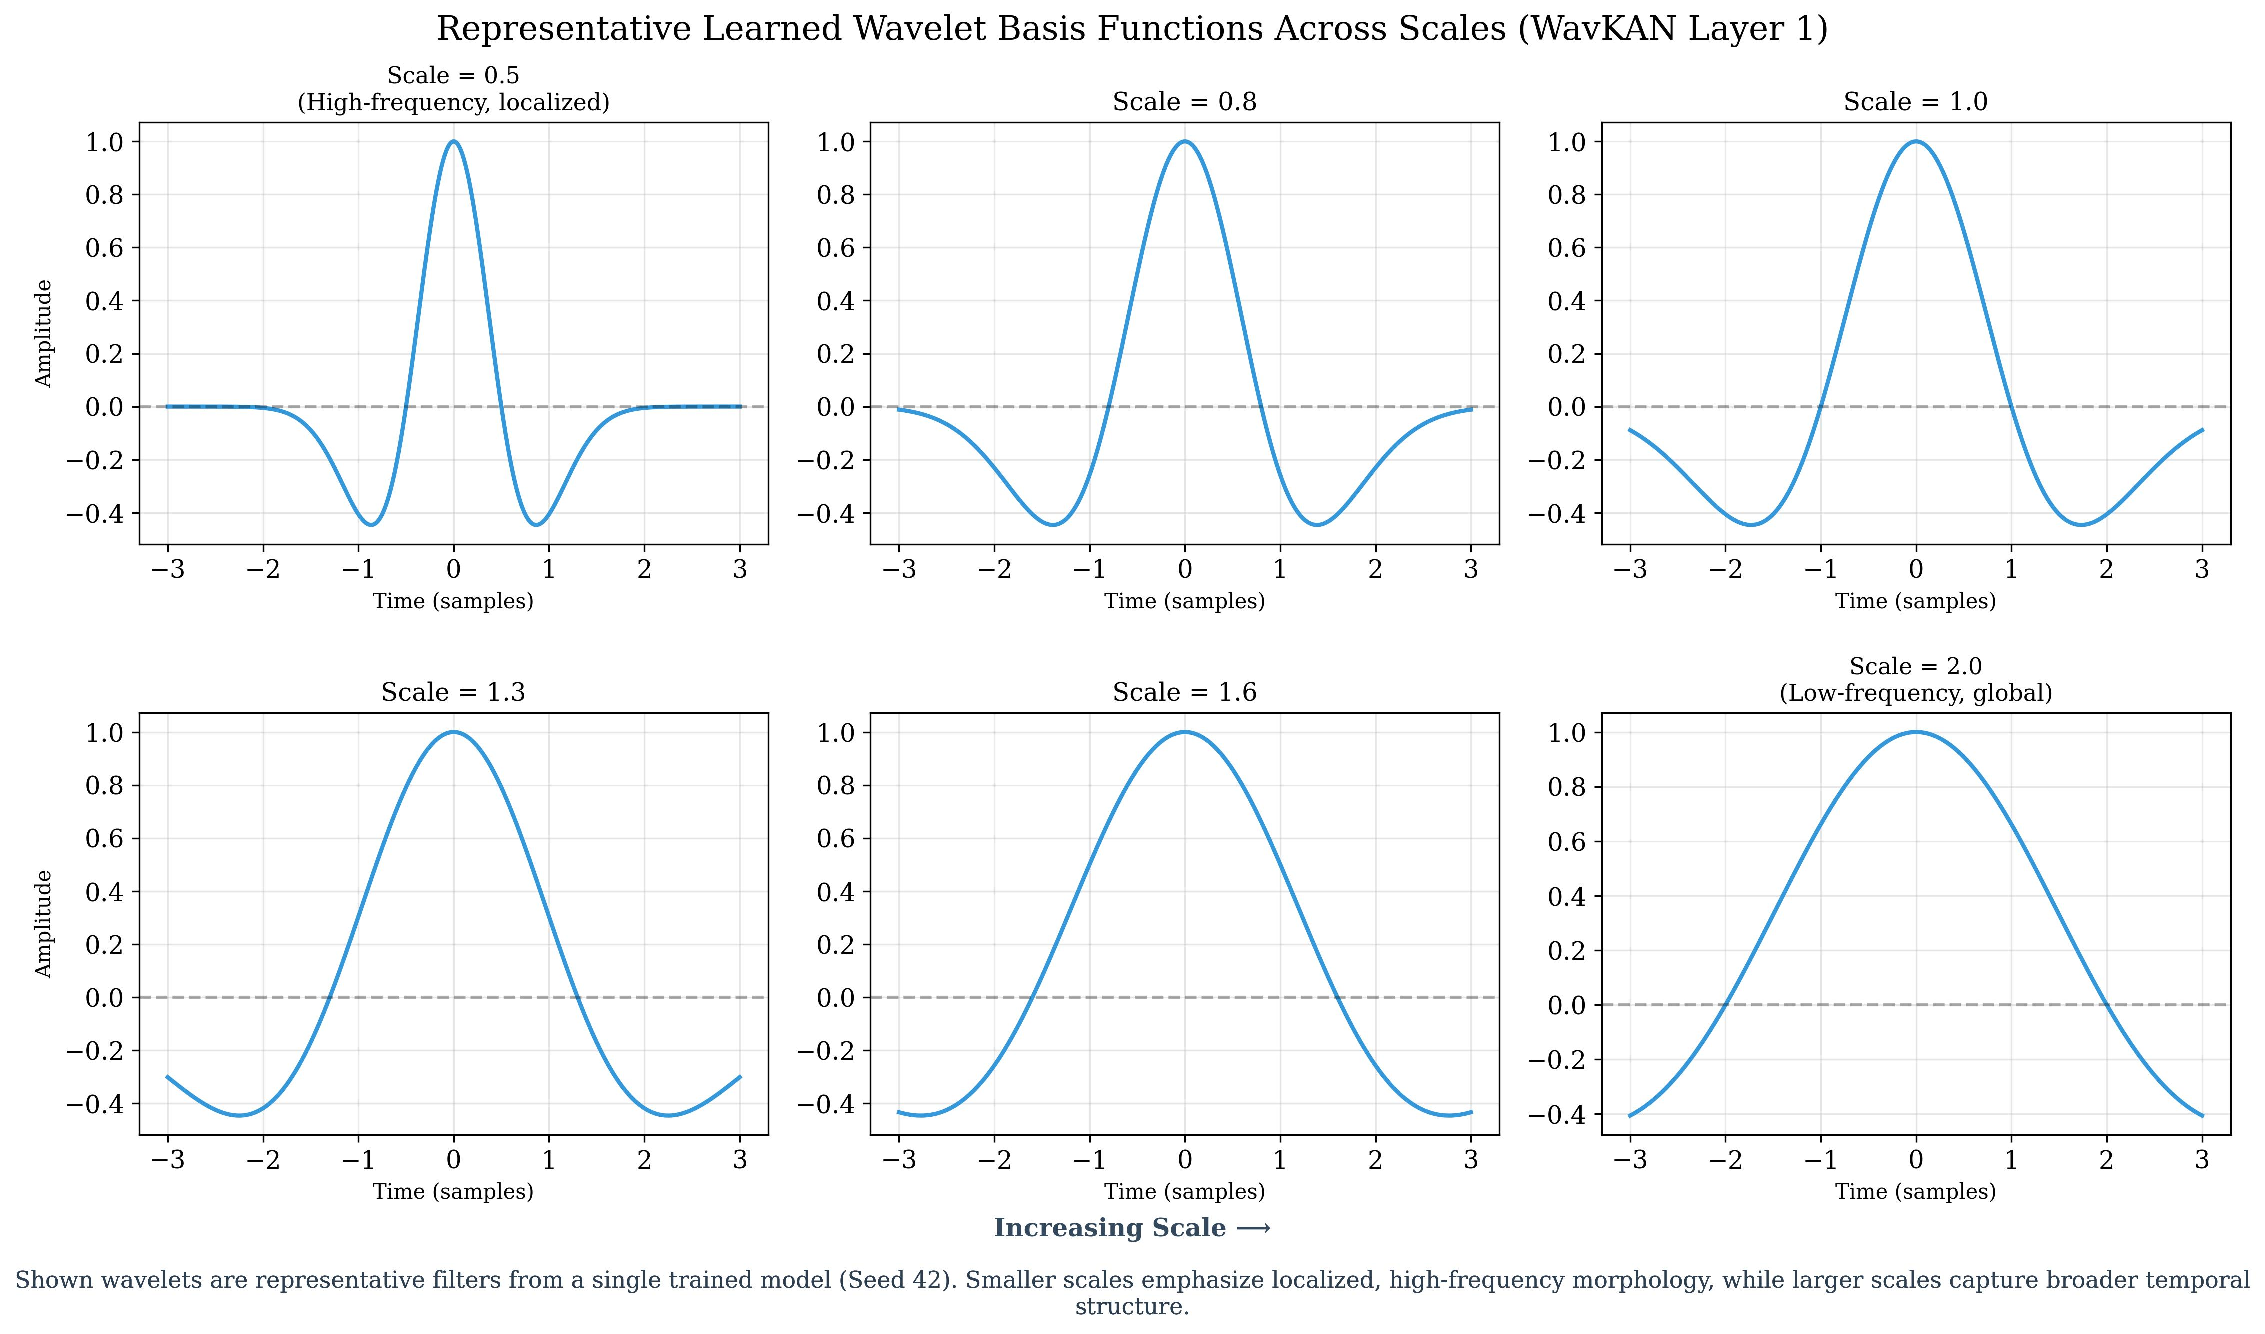
\includegraphics[width=\textwidth]{final_learned_wavelets.pdf}
\caption{\textbf{Interpretability: Learned Wavelet Bases.} WavKAN learns adaptive Mexican Hat wavelets (blue curves) that align with specific morphological features.}
\label{fig:wavelets}
\end{figure}

\textbf{Lightweight and Edge Deployable ECG Models:} The development of resource efficient classifiers for ECG is important for wearable health monitoring. Farag \cite{farag_tiny_2023} has demonstrated that miniature matched-filter CNNs can be employed for competitive performance with substantially reduced computational cost ($\approx 15$ KB). Similarly, Elsheikhy et al. \cite{elsheikhy_lightweight_2025} demonstrated the need for lightweight architectures for edge deployment. Our work is in line with this Green AI paradigm. WavKAN-CL achieves a Ventricular (V) recall of 0.86---which is similar to deep baselines such as Guo et al. \cite{guo_inter-patient_2019}, but using only 95k parameters.

This corresponds to a $> 90\%$ reduction in parameter count relative to conventional DenseNet or Transformer architectures, prioritizing ventricular event detection and deployment feasibility over marginal gains in minority-class sensitivity.

%% 8. CONCLUSION
\section{Conclusion}
\label{sec:conclusion}
This paper proposed WavKAN-CL, a structurally transparent and parameter efficient arrhythmia classification framework. By replacing fixed activation functions of standard MLPs with learnable Mexican Hat wavelets, the model enables representations that are related to the morphology of the QRS complex, thus solving the black box interpretability challenge \cite{taleban_explainable_2026}. Evaluated on a strict inter-patient protocol (DS1/DS2 split) WavKAN-CL gives a mean Ventricular (V) recall of 0.88 over 20 seeds (peak 0.93), while using only 95,189 parameters. This is a $>95\%$ reduction in size when compared to the Transformer-based architectures and supporting its suitability for battery-constrained wearable devices \cite{farag_tiny_2023}. The discrimination of minority Supraventricular (S) beats remains challenging under non-augmented inter-patient schemes \cite{bahrami_investigation_2025}, whereas the proposed curriculum learning strategy significantly reduces the generalization gap to $\le 0.01$. Future work will focus on incorporating P-wave specific attention heads to resolve S-beat ambiguity and deploying the quantized model on low-power edge hardware. These results demonstrate that wavelet-based networks with structural interpretability provide a good alternative for large black-box models for safety-critical biomedical applications.

\backmatter

\section*{Declarations}

\textbf{Funding:} Article Processing Charge (APC) of this manuscript was funded by the Vellore Institute of Technology (VIT).

\textbf{Conflict of Interest:} The authors declare that they have no known competing personal interests or relationships that may have perceived influence on the work reported in this paper;

\textbf{CRediT Author Statement:} 
\textbf{Venkate Ramanan Manivannan:} Conceptualization, Methodology, Software, Validation, Formal Analysis, Writing - Original Draft, Visualization. 
\textbf{Ramanathan Lakshmanan:} Conceptualization, Resources, Validation, Supervision, Project Administration, Writing - Review \& Editing.

\textbf{Data Availability:} The datasets analyzed during the current study (MIT-BIH Arrhythmia Database) are publicly available in the PhysioNet repository: \url{https://physionet.org/content/mitdb/1.0.0/} \cite{moody_mit-bih_1992}.

\textbf{Code Availability:} Source code and pre-trained weights are available at: \url{https://github.com/vrhsr/WavKAN-CL}.

\bibliography{references}

\end{document}
